\documentclass[12pt]{article}


% -------------------- PAQUETES --------------------
\usepackage[utf8]{inputenc}
\usepackage[spanish]{babel}
\usepackage[margin=2.54cm]{geometry}
\usepackage{graphicx}
\usepackage{xcolor}
\usepackage{enumitem}
\usepackage{parskip}
\usepackage{hyperref}
\usepackage{ulem} 
\usepackage{subcaption}
\usepackage{xurl}


% -------------------- CARGA DE ARCHIVOS EXTERNOS --------------------
% ----------------- UTILIDADES PARA DAR UN MEJOR FORMATO DE DOCUMENTO -----------------  


\definecolor{azul}{rgb}{0.0039, 0.3098, 0.6196}


% Formato para el indice general ...........
\makeatletter
    \renewcommand{\@dotsep}{1.5}
    \renewcommand{\l@section}{\@dottedtocline{1}{1.5em}{2.3em}}
    \renewcommand{\l@subsection}{\@dottedtocline{2}{3.8em}{3.2em}}
    \renewcommand{\l@subsubsection}{\@dottedtocline{3}{7.0em}{4.1em}}
\makeatother

% --------- COMANDOS PERSONALIZADOS PARA LA PORTADA DE LAS TAREAS, TRABAJOS Y PROYECTOS ---------

\newcommand{\rutaLogo}[1]{\newcommand{\RutaLogo}{#1}}
\newcommand{\tema}[1]{\newcommand{\Tema}{#1}}
\newcommand{\etiquetaAutores}[1]{\newcommand{\EtiquetaAutores}{#1}}
\newcommand{\alumno}[1]{\newcommand{\Alumno}{#1}}
\newcommand{\materia}[1]{\newcommand{\Materia}{#1}}
\newcommand{\docente}[1]{\newcommand{\Docente}{#1}}
\newcommand{\ciclo}[1]{\newcommand{\Ciclo}{#1}}
\newcommand{\fecha}[1]{\newcommand{\Fecha}{#1}}
\newcommand{\periodo}[1]{\newcommand{\Periodo}{#1}}



% -------------------- DEFINICIÓN DE LA PORTADA --------------------
\rutaLogo{../../docs/img/logo-ista.png}
\tema{\\ \vspace{0.5cm} Formas de navegar por internet \\ \vspace{1.2cm}}
\etiquetaAutores{Alumno:}
\alumno{Eduardo Mendieta \vspace{0.7cm}}
\materia{Ofimática \vspace{0.7cm}}
\docente{Ing. Jessica Herrera, Mgtr.\vspace{0.7cm}}
\ciclo{Primer Ciclo \vspace{0.7cm}}
\fecha{12 de agosto de 2024 \vspace{0.7cm}}
\periodo{Abril 2024 - Agosto 2024}

\begin{document}

        \begin{titlepage}

    \centering

    \includegraphics[width=0.11\textwidth]{\RutaLogo} 

    \vspace{0.3cm}
    \textcolor{azul}{\Large \textbf{Instituto Superior Universitario Tecnológico del Azuay \\}}
    \vspace{0.3cm}
    \textcolor{azul}{\Large \textbf{Tecnología Superior en Big Data}}
    
    % 1. ---------------- TEMA -------------------------
    
    {\Large\textbf{\Tema}}
    
    % 2. ---------------- AUTOR(ES) -------------------------
    \textcolor{azul}{\large \textbf{\EtiquetaAutores} \\}
    \vspace{0.3cm}
    {\large \Alumno}

    % 3. ---------------- MATERIA -------------------------
    \textcolor{azul}{\large \textbf{Materia:} \\}
    \vspace{0.3cm}
    {\large \Materia}


    % 3. ---------------- DOCENTE -------------------------
    \textcolor{azul}{\large \textbf{Docente:} \\}
    \vspace{0.3cm}
    {\large \Docente}


    % 3. ---------------- Ciclo -------------------------
    \textcolor{azul}{\large \textbf{Ciclo:} \\}
    \vspace{0.3cm}
    {\large \Ciclo}


    % 3. ---------------- FECHA -------------------------
    \textcolor{azul}{\large \textbf{Fecha:} \\}
    \vspace{0.3cm}
    {\large \Fecha}

    % 3. ---------------- PERIODO -------------------------
    \textcolor{azul}{\large \textbf{Periodo Académico:} \\}
    \vspace{0.3cm}
    {\large \Periodo}
 
\end{titlepage}


        \tableofcontents
        \newpage

        \section*{\centering Formas de navegar por internet} \vspace{.5cm}

        % 1.Introducción: ...................................................
        \section{Introducción}
                La navegación por internet es un proceso técnico que implica la interacción con una variedad de tecnologías y protocolos fundamentales para la transferencia y visualización de información en la red. Este proceso se basa en la utilización del protocolo HTTP/HTTPS, la resolución de nombres de dominio a través del DNS, y la gestión de datos en formatos como HTML, CSS y JavaScript.

                En el ámbito de la ofimática, la navegación por internet es una herramienta clave para acceder a plataformas de productividad en la nube, como suites ofimáticas, herramientas de colaboración y servicios de gestión de proyectos. Estas plataformas requieren que los usuarios naveguen entre interfaces, gestionen documentos en línea y utilicen aplicaciones que integran servicios en la web con software local, optimizando así los flujos de trabajo.
                
                En el contexto del Big Data, la navegación por internet se convierte en una fuente rica de datos no estructurados y semi-estructurados. Cada interacción en la web, como clics y búsquedas, genera un rastro digital que puede ser capturado, almacenado y analizado. La minería de datos y los algoritmos avanzados permiten extraer información valiosa de estos datos, convirtiendo la navegación en una actividad crucial para el enriquecimiento de bases de datos masivas. Además, la interacción con grandes volúmenes de datos en tiempo real a través de plataformas web es esencial para la toma de decisiones informadas en diversos sectores.


        % 2.Objetivos: ...................................................
        \section{Objetivos}
                \subsection{Objetivo general}
                        Investigar sobre las diferentes formas que existen para navegar por Internet.

                \subsection{Objetivos específicos}
                        \begin{itemize}
                                \item Utilizar métodos utilizados en clase apara agilizar las busquedas sobre el tema.
                                \item Recopilar información que permita entender las diferentes formas que existen de navegar en Internet.
                        \end{itemize}


        % 3.Marco Teórico: ...................................................
        \newpage
        \section{Marco Teórico}
                El acceso y la navegación por internet son fundamentales en el contexto contemporáneo, donde la conectividad digital influye en casi todos los aspectos de la vida moderna. La forma en que los usuarios interactúan con la web ha evolucionado significativamente, dando lugar a diversas metodologías y herramientas que facilitan la exploración y el uso de los recursos en línea.

                En este marco, resulta esencial comprender las distintas maneras en que se puede navegar en internet, ya que cada método ofrece características particulares que responden a necesidades específicas. Estas formas de navegación no solo reflejan la diversidad de dispositivos y plataformas disponibles, sino también las preferencias individuales y las consideraciones de seguridad y privacidad que los usuarios deben tener en cuenta.

                A continuación, se describen las principales formas de navegar en internet, abarcando desde los métodos tradicionales hasta las opciones más avanzadas y especializadas.
                
                \subsection{Navegadores web}
                        Los navegadores web operan sobre la base del Protocolo de Transferencia de Hipertexto (HTTP) y su versión segura (HTTPS). Cuando un usuario ingresa una dirección web (URL) en la barra de direcciones del navegador, este envía una solicitud al servidor web correspondiente. El servidor, a su vez, responde enviando el contenido solicitado, que el navegador interpreta y muestra al usuario. Este proceso incluye la descarga de archivos HTML, hojas de estilo CSS, y scripts JavaScript, que en conjunto crean la experiencia visual y funcional de la página web.

                        \textbf{Funcionalidades comunes de los navegadores web:}

                        \begin{itemize}
                                \item Permiten ingresar URLs para acceder a diferentes sitios web.
                                \item Facilitan la apertura de múltiples páginas web dentro de una sola ventana del navegador, mejorando la organización y eficiencia.
                                \item Ofrecen la posibilidad de guardar direcciones web para un acceso rápido en el futuro.
                                \item Registran las páginas web visitadas anteriormente, permitiendo a los usuarios volver a sitios de interés.
                                \item Añaden funcionalidades adicionales al navegador, como bloqueadores de anuncios, gestores de contraseñas y herramientas de productividad.
                        \end{itemize}

                        Los navegadores modernos implementan diversas medidas para proteger a los usuarios de amenazas como malware, phishing y ataques de sitios web maliciosos. Entre estas medidas se incluyen la navegación en modo incógnito, que no guarda el historial de navegación ni las cookies, y el uso de certificados SSL para asegurar las conexiones entre el navegador y los sitios web. Además, los usuarios deben estar atentos a las configuraciones de privacidad y las actualizaciones de seguridad para proteger sus datos personales.

                        Existen varios navegadores web populares, cada uno con sus propias características y ventajas. Entre los más utilizados se encuentran Google Chrome, Mozilla Firefox, Microsoft Edge y Safari. Cada navegador ofrece una combinación única de velocidad, compatibilidad con estándares web, y características de seguridad, lo que permite a los usuarios elegir el que mejor se adapte a sus necesidades y preferencias.

                \subsection{Aplicaciones móviles}
                        Las aplicaciones móviles para navegación web, como navegadores específicos o aplicaciones de contenido, operan de manera similar a los navegadores web de escritorio, pero están optimizadas para la experiencia móvil. Estos programas utilizan protocolos como HTTP y HTTPS para conectar con servidores web, mostrar contenido y permitir interacciones. Las aplicaciones móviles están diseñadas para aprovechar las características específicas de los dispositivos, como pantallas táctiles, sensores de ubicación y capacidades de cámara, para ofrecer una experiencia de usuario más integrada y personalizada.

                        \textbf{Ventajas:}

                        \begin{itemize}
                                \item Las aplicaciones móviles permiten acceder a Internet desde cualquier lugar, siempre que haya conexión a la red, ofreciendo una gran flexibilidad y conveniencia.
                                \item Muchas aplicaciones están diseñadas para proporcionar una experiencia adaptada a las necesidades y preferencias del usuario, como notificaciones push, contenido recomendado y ajustes personalizados.
                                \item Suelen integrarse bien con otras funciones del dispositivo, como la cámara, el GPS y los contactos, facilitando una navegación más fluida y funcional.
                                \item Están diseñadas para aprovechar las características del hardware del dispositivo, como pantallas táctiles y tamaños de pantalla variados, proporcionando una interfaz de usuario optimizada para la interacción móvil.
                        \end{itemize}

                        \textbf{Desventajas:}

                        \begin{itemize}
                                \item Pueden consumir considerablemente más recursos del dispositivo, como memoria y batería, especialmente si se ejecutan en segundo plano.
                                \item Las aplicaciones requieren actualizaciones regulares para mantenerse seguras y funcionales. Además, pueden enfrentar problemas de compatibilidad con diferentes versiones de sistemas operativos y dispositivos.
                        \end{itemize}

                        La importancia de las aplicaciones móviles para navegar por Internet radica en su capacidad para ofrecer una experiencia de usuario adaptada a las necesidades y comportamientos móviles. La facilidad de uso es una característica clave, ya que las aplicaciones suelen estar diseñadas con interfaces intuitivas y funcionalidades accesibles, aprovechando el diseño centrado en el usuario para facilitar la navegación y la interacción.

                        A pesar de su facilidad de uso y adaptabilidad, la factibilidad de utilizar aplicaciones móviles para navegar por Internet depende de varios factores críticos. La calidad de la conexión a Internet, la capacidad del dispositivo y las preferencias del usuario juegan un papel fundamental en el rendimiento de estas aplicaciones. Por lo tanto, es esencial que las aplicaciones sean desarrolladas con atención a estos aspectos para asegurar un funcionamiento óptimo en diversas condiciones. Además, la protección de la privacidad y seguridad de los datos personales es crucial; los usuarios deben asegurarse de que las aplicaciones sean confiables y cuenten con medidas adecuadas de protección de datos para garantizar una navegación segura y eficiente.


                \subsection{Navegación por línea de comandos}
                        La línea de comandos, o terminal, es una interfaz de texto que permite a los usuarios interactuar con el sistema operativo de un computador mediante la entrada de comandos escritos. A diferencia de las interfaces gráficas de usuario, que utilizan ventanas, iconos y menús, la línea de comandos requiere que los usuarios escriban comandos específicos para realizar tareas.
                        
                        \textbf{Herramientas de navegación por internet a través de línea de comandos:}

                        \begin{enumerate}
                                \item \textbf{Lynx:} Es un navegador web basado en texto que permite a los usuarios navegar por Internet desde la línea de comandos. A diferencia de los navegadores gráficos, Lynx no muestra imágenes ni gráficos; en su lugar, muestra el contenido de las páginas web en formato de texto. Esto puede ser útil para usuarios con conexiones lentas o para aquellos que prefieren una interfaz más sencilla. Lynx también es beneficioso para la accesibilidad, ya que facilita la navegación a personas con discapacidades visuales que utilizan lectores de pantalla.
                                \item \textbf{Wget:} Es una herramienta diseñada para descargar contenido desde la web. Permite a los usuarios obtener archivos, sitios web completos o partes de estos de manera automática desde la línea de comandos. Wget es especialmente útil para descargar grandes cantidades de datos, hacer copias de seguridad de sitios web o recuperar contenido de manera rápida y eficiente. A través de Wget, se pueden especificar opciones para controlar cómo se realizan las descargas, como el límite de velocidad, el número de intentos en caso de fallo, y la profundidad de la descarga de enlaces.
                                \item \textbf{Curl:} Es una herramienta versátil que se utiliza para transferir datos entre un cliente y un servidor a través de varios protocolos, como HTTP, HTTPS, FTP y otros. A diferencia de Wget, que está más centrado en la descarga de archivos, Curl es útil para realizar solicitudes web más complejas, como enviar datos a un servidor, interactuar con APIs y obtener información detallada sobre las respuestas del servidor. Curl proporciona una gran flexibilidad en el manejo de solicitudes y respuestas, permitiendo a los usuarios ajustar los parámetros de sus solicitudes para obtener exactamente la información que necesitan.
                        \end{enumerate}

                        \textbf{Ventajas de utilizar herramientas de línea de comandos:}

                        \begin{itemize}
                                \item Las herramientas de línea de comandos suelen ser más rápidas y menos exigentes en términos de recursos del sistema, lo que permite realizar tareas de manera eficiente incluso en sistemas con hardware limitado.
                                \item Estas herramientas permiten la automatización de tareas repetitivas mediante la creación de scripts, lo que facilita la gestión de grandes volúmenes de datos o la realización de tareas programadas.
                                \item Para usuarios que prefieren una interfaz sin distracciones o necesitan herramientas que funcionen en entornos de servidor sin interfaces gráficas, las herramientas de línea de comandos ofrecen una solución accesible y sencilla.
                        \end{itemize}

                        \textbf{Desventajas:}

                        \begin{itemize}
                                \item La línea de comandos puede parecer intimidante para aquellos que están acostumbrados a interfaces gráficas. Requiere aprender y recordar una serie de comandos y opciones.
                                \item A diferencia de los navegadores gráficos, las herramientas de línea de comandos no ofrecen una experiencia visual rica, lo que puede limitar la interacción con contenido web que incluye imágenes y otros elementos multimedia.
                        \end{itemize}


                \subsection{Otros dispositivos}
                        Con el avance de la tecnología, ahora es posible explorar la web desde televisores y consolas de videojuegos, ampliando así las formas en que interactuamos con contenido en línea, dejado de ser una actividad exclusiva de computadoras y dispositivos móviles.

                        \textbf{Televisores:}
                        
                        Los televisores inteligentes, o Smart TVs, han revolucionado la manera en que consumimos contenido en casa. Equipados con sistemas operativos propios y conectividad a Internet, estos televisores permiten a los usuarios acceder a una variedad de aplicaciones y servicios en línea directamente desde la pantalla grande de su televisor.
                       
                        Muchos televisores inteligentes incluyen navegadores web preinstalados o permiten la instalación de aplicaciones de navegación. Estos navegadores funcionan de manera similar a los de computadoras y dispositivos móviles, aunque con interfaces adaptadas para el control remoto del televisor. La navegación web en una Smart TV ofrece una experiencia visual inmersiva, ideal para explorar contenido multimedia, leer noticias o realizar búsquedas generales en la web desde la comodidad del salón.

                        Además de la navegación web tradicional, los televisores inteligentes ofrecen acceso a aplicaciones de streaming como Netflix, YouTube y Amazon Prime Video. Estas aplicaciones permiten a los usuarios ver series, películas y videos en alta definición, aprovechando las capacidades de resolución y sonido del televisor. La integración con servicios en línea amplía la funcionalidad del televisor, haciendo que sea una herramienta versátil para el entretenimiento digital.

                        \textbf{Consolas de videojuegos:}

                        Las consolas de videojuegos modernas, como PlayStation, Xbox y Nintendo Switch, han evolucionado más allá de ser simples dispositivos de entretenimiento. Equipadas con conectividad a Internet y aplicaciones integradas, estas consolas también permiten a los usuarios navegar por la web y acceder a una variedad de servicios en línea.

                        Incluyen navegadores web integrados que permiten a los usuarios explorar Internet mientras están en modo de juego o en la pantalla de inicio. Al igual que en los navegadores de computadoras, estos navegadores permiten acceder a sitios web, realizar búsquedas y explorar contenido en línea. La experiencia de navegación puede variar según la consola y el navegador integrado, pero generalmente ofrece una interfaz simplificada adaptada para el uso con un control de videojuego.

                        Al igual que los televisores inteligentes, las consolas de videojuegos ofrecen acceso a aplicaciones de streaming y otros servicios en línea. Los usuarios pueden ver películas y series, escuchar música y participar en redes sociales a través de aplicaciones específicas disponibles en la tienda de la consola. Estas aplicaciones están diseñadas para integrarse con la experiencia de juego y el entretenimiento general, proporcionando una plataforma multifuncional.

                        \textbf{Ventajas:}

                        \begin{itemize}
                                \item Navegar por Internet en un televisor inteligente o consola de videojuegos ofrece una experiencia visual más grande y envolvente en comparación con dispositivos móviles o computadoras.
                                \item La integración de servicios en línea en televisores y consolas permite a los usuarios acceder a múltiples tipos de contenido desde un solo dispositivo, reduciendo la necesidad de cambiar entre diferentes aparatos.
                                \item Estas tecnologías permiten a los usuarios acceder a la web y a servicios digitales desde el salón o el espacio de juego, lo que puede ser especialmente conveniente para actividades sociales o familiares.
                        \end{itemize}


                        \textbf{Limitaciones:}

                        \begin{itemize}
                                \item La navegación en televisores y consolas puede ser menos fluida y más complicada debido al uso de controles remotos o joysticks en lugar de teclado y ratón, lo que puede dificultar la interacción con algunos sitios web o aplicaciones.
                                \item Aunque las consolas y televisores inteligentes han avanzado, sus navegadores web y aplicaciones pueden no ofrecer la misma funcionalidad completa o la misma velocidad que los navegadores de computadoras y dispositivos móviles.
                        \end{itemize}

                \subsection{Navegación automatizada}

                la navegación por Internet no se limita a la interacción manual a través de navegadores gráficos; también involucra técnicas automatizadas que pueden optimizar y expandir las capacidades de recolección y análisis de datos. Entre estas técnicas se encuentran los bots, los scripts y el web scraping, herramientas esenciales para profesionales en el campo del análisis de datos y la ciencia de datos. 

                Los bots, o robots de software, son programas automatizados diseñados para realizar tareas específicas en la web de manera repetitiva y eficiente. Pueden ser configurados para llevar a cabo una amplia gama de actividades, desde realizar búsquedas en Internet hasta interactuar con páginas web y recoger datos. Los bots son especialmente útiles para tareas que requieren precisión y consistencia, como la recopilación de información de múltiples fuentes o la monitorización de cambios en sitios web.

                Los scripts son secuencias de comandos programados para ejecutar tareas automáticas en sistemas informáticos. En el contexto de la navegación por Internet, los scripts se utilizan para interactuar con páginas web, enviar datos, y realizar acciones como clics y desplazamientos. Los scripts pueden ser escritos en varios lenguajes de programación, como Python, JavaScript o Bash, y son fundamentales para la personalización de la automatización de tareas específicas en la web. Los scripts permiten a los usuarios automatizar procesos complejos y reducir el tiempo necesario para completar tareas repetitivas.

                El web scraping es una técnica que utiliza bots y scripts para extraer información de páginas web de manera automatizada. Consiste en recorrer sitios web y recolectar datos específicos, como texto, imágenes o enlaces, para almacenarlos y analizarlos posteriormente. Esta técnica es esencial para obtener grandes volúmenes de datos de diversas fuentes en línea, facilitando el análisis y la generación de insights valiosos. El web scraping puede realizarse utilizando herramientas y bibliotecas especializadas, como BeautifulSoup o Scrapy en Python, que permiten extraer y procesar datos de manera eficiente.

                Los bots a menudo utilizan scripts para ejecutar tareas específicas en la web, mientras que el web scraping se basa en bots y scripts para extraer información de manera automatizada. Esta combinación permite a los profesionales automatizar la recolección y el análisis de datos, facilitando la gestión de grandes volúmenes de información y optimizando la toma de decisiones basada en datos.

                Para los analistas de datos y científicos de datos, la capacidad de utilizar bots, scripts y técnicas de web scraping es crucial para acceder y procesar datos de manera eficiente. Estas herramientas permiten:

                \begin{itemize}
                        \item Automatizar la recolección de datos de múltiples fuentes en línea, reduciendo el tiempo y esfuerzo necesarios para obtener información relevante.
                        \item Facilitar el manejo y análisis de grandes conjuntos de datos que son esenciales para la toma de decisiones informadas y la generación de insights valiosos.
                        \item Permitir la monitorización continua de sitios web y la actualización automática de datos, asegurando que la información utilizada esté siempre actualizada y sea precisa.
                \end{itemize}


        
                
          % 4.Evidencias: ...................................................
        \newpage
        \section{Evidencias de busqueda utilizando métodos y operadores}      
                
                \begin{figure}[h!]
                        \centering
                        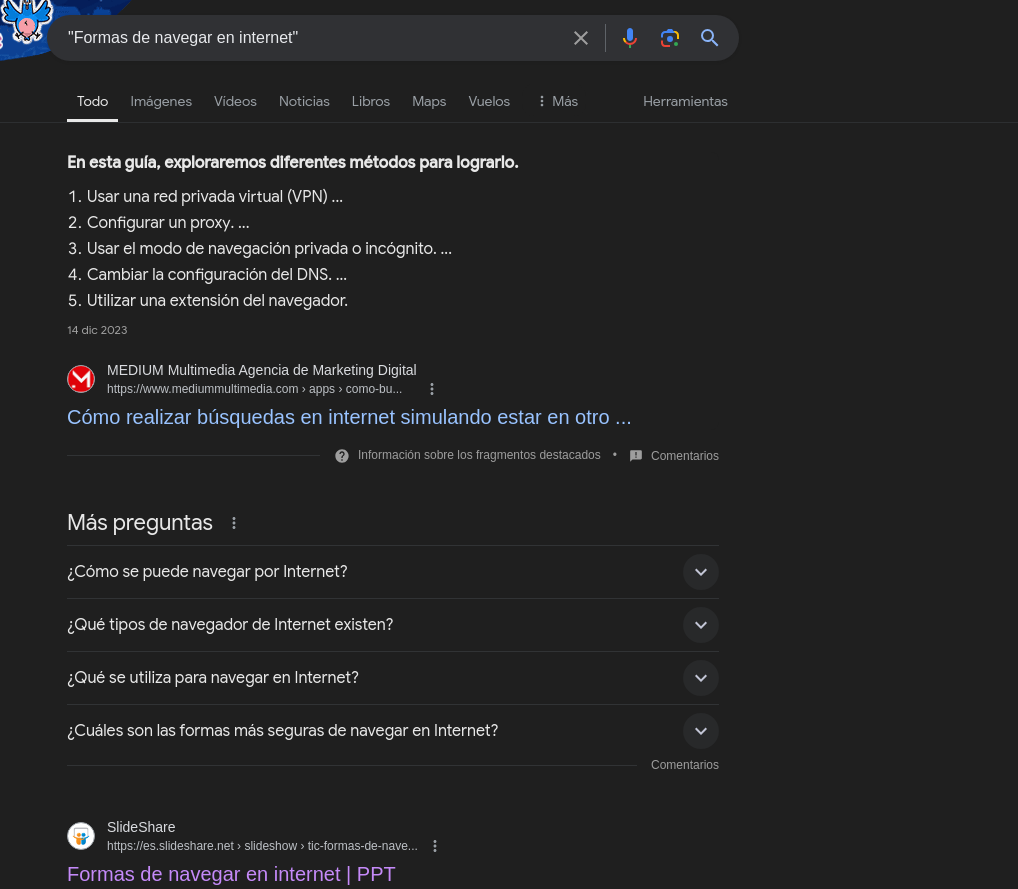
\includegraphics[width=0.7\textwidth]{img/t1-1.png}
                        \caption{Busqueda utilizando comillas}
                \end{figure}

                \begin{figure}[h!]
                        \centering
                        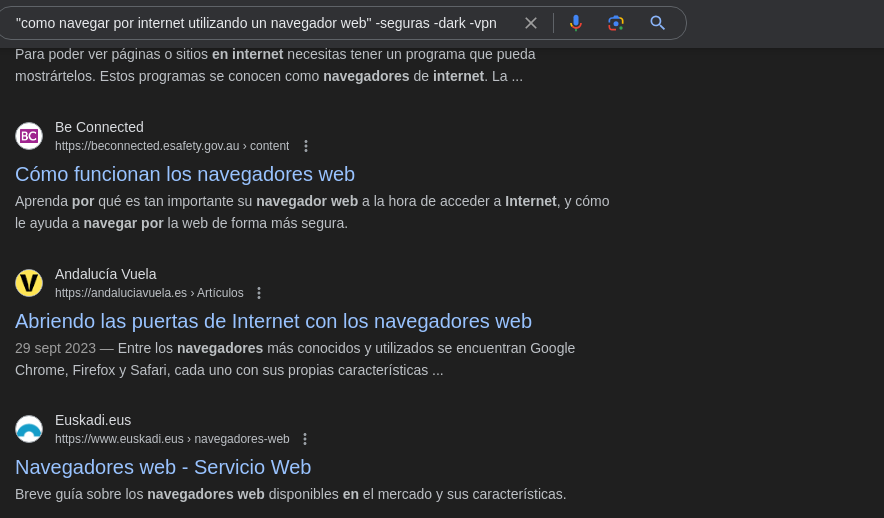
\includegraphics[width=0.7\textwidth]{img/t1-2.png}
                        \caption{Busqueda utilizando comillas y excluyendo términos}
                \end{figure}

                \newpage
                \begin{figure}[h!]
                        \centering
                        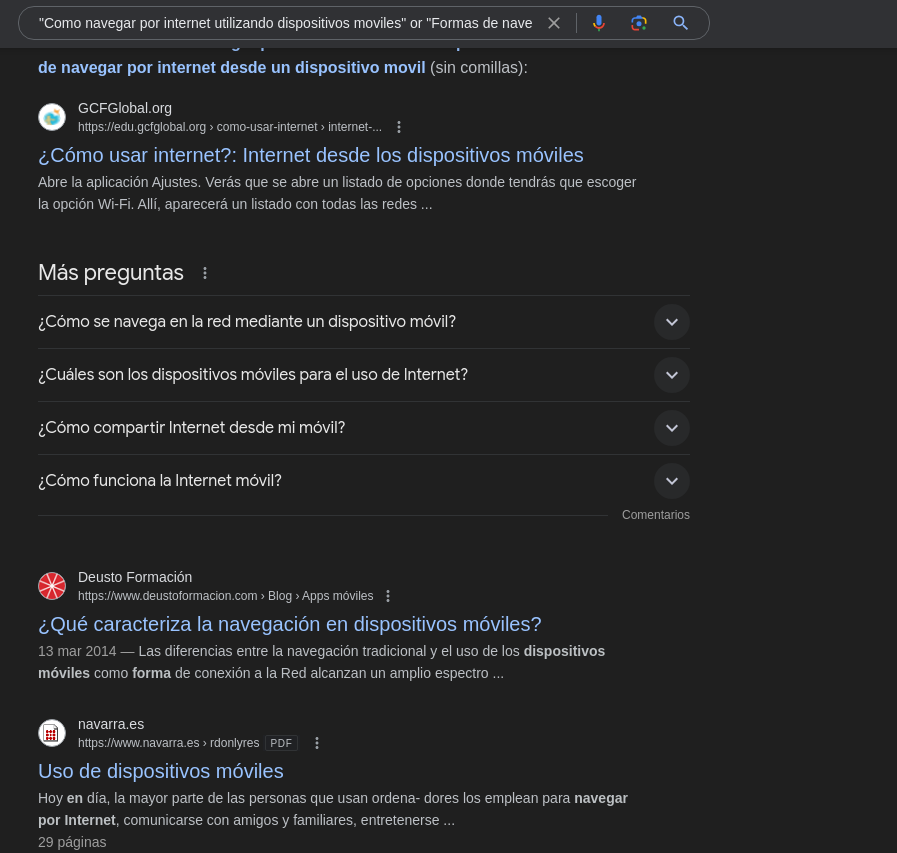
\includegraphics[width=0.7\textwidth]{img/t1-3.png}
                        \caption{Busqueda operadores como \textit{OR}}
                \end{figure}

                \begin{figure}[h!]
                        \centering
                        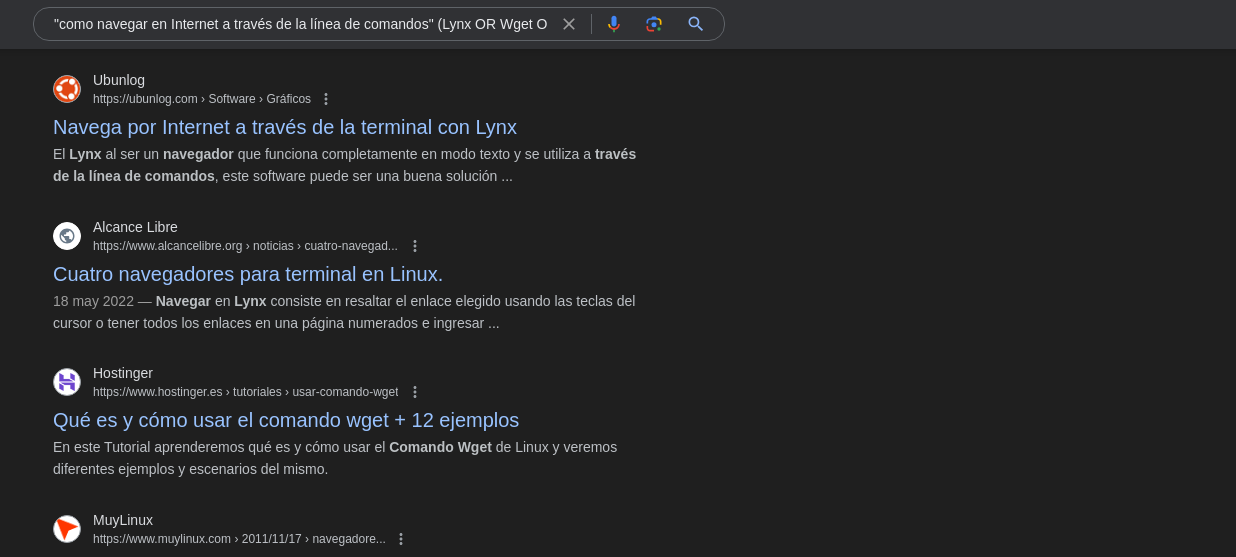
\includegraphics[width=0.9\textwidth]{img/t1-4.png}
                        \caption{Realizando una búsqueda centrada utilizando \textit{OR}}
                \end{figure}

                \begin{figure}[h!]
                        \centering
                        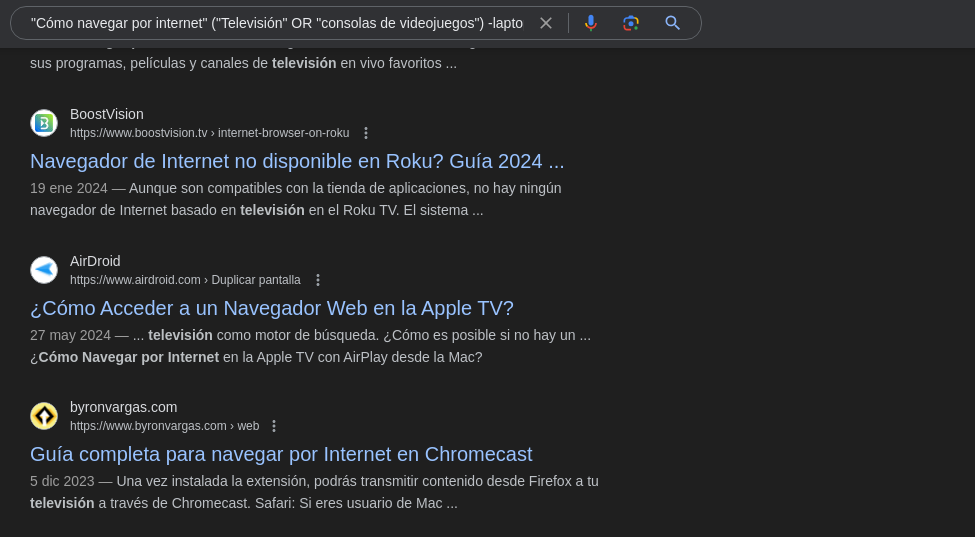
\includegraphics[width=0.7\textwidth]{img/t1-5.png}
                        \caption{Realizando una búsqueda centrada utilizando \textit{OR} y excluyendo terminos}
                \end{figure}

                \begin{figure}[h!]
                        \centering
                        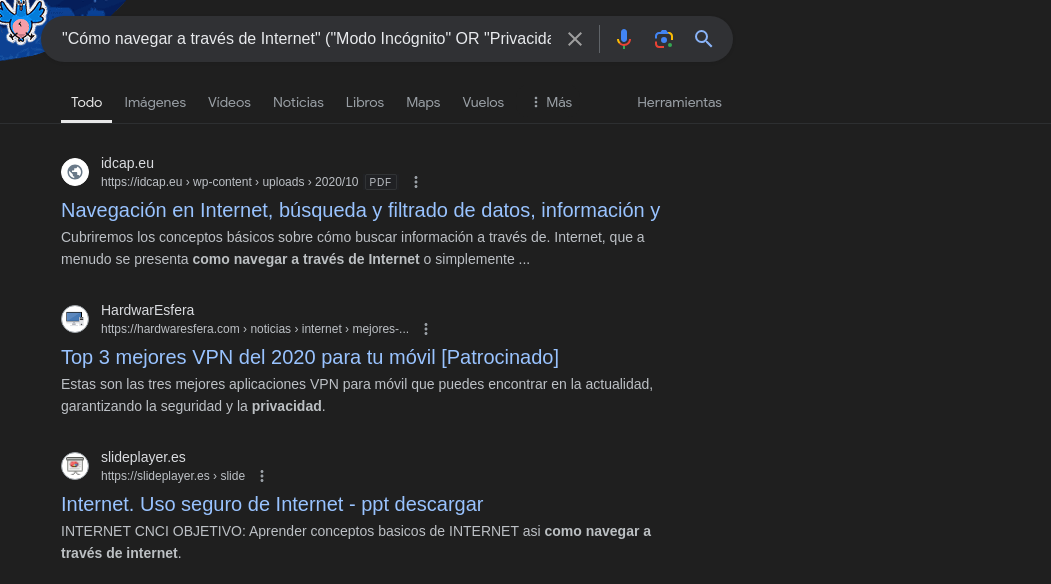
\includegraphics[width=0.7\textwidth]{img/t1-6.png}
                        \caption{Realizando una búsqueda centrada utilizando \textit{OR}}
                \end{figure}

                \begin{figure}[h!]
                        \centering
                        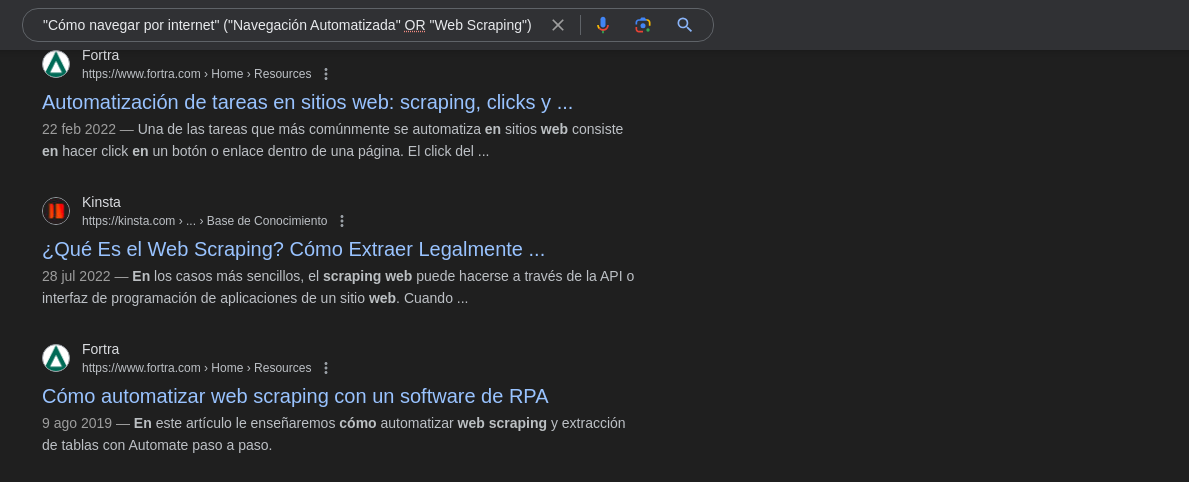
\includegraphics[width=0.8\textwidth]{img/t1-7.png}
                        \caption{Realizando una búsqueda centrada utilizando \textit{OR}}
                \end{figure}
                

        % 5.Conclusiones: ...................................................
        \newpage
        \section{Conclusiones}
            \begin{enumerate}
                \item La navegación web ha avanzado desde el uso básico de HTTP/HTTPS hasta la integración con plataformas de productividad en la nube y la gestión de datos en Big Data.
                \item La navegación en Internet abarca diversos métodos, como navegadores web y aplicaciones móviles, adaptándose a diferentes tecnologías y necesidades, desde la transferencia de información hasta la interacción con plataformas de productividad.
                \item Los navegadores web facilitan el acceso y la visualización de información, mientras que las aplicaciones móviles ofrecen acceso conveniente pero pueden enfrentar desafíos en términos de consumo de recursos.
                \item Bots, scripts y web scraping son herramientas clave para capturar y analizar datos generados por la navegación web, esencial para el enriquecimiento de bases de datos masivas en el contexto del Big Data.
                \item Aunque los televisores inteligentes y consolas ofrecen una experiencia visual amplia para la navegación web, pueden ser menos funcionales en comparación con dispositivos tradicionales debido a limitaciones en la interfaz y la velocidad.
            \end{enumerate}

        % 6.Bibliografía: ...................................................
        \newpage
        \section{Bibliografía}
        \begin{itemize}
                \item Bilichenko, E. (2023, 14 febrero). Navegación del sitio web: definición e importancia. Blog Netcommerce. \url{https://info.netcommerce.mx/navegacion/}
                \item Vasco, E. J.-G., \& Vasco, E. J.-G. (s. f.). Navegadores web - Servicio Web - Euskadi.eus. Eusko Jaurlaritza - Gobierno Vasco. \url{https://www.euskadi.eus/navegadores-web/web01-a2wz/es/}
                \item ¿Qué es un navegador web y cómo funciona? - cdmon. (s. f.). Cdmon. \url{https://www.cdmon.com/es/blog/que-es-un-navegador-y-como-funciona}
                \item Colaboradores de Wikipedia. (2023, 30 junio). Navegador móvil. Wikipedia, la Enciclopedia Libre. \url{https://es.wikipedia.org/wiki/Navegador_m%C3%B3vil}
                \item Darkcrizt. (2018b, diciembre 3). ¿Cómo navegar por la web desde la terminal de Linux? Desde Linux. \url{https://blog.desdelinux.net/como-navegar-por-la-web-desde-la-terminal-de-linux/}
                \item Darkcrizt. (2018, 25 mayo). Navega por Internet a través de la terminal con Lynx. Ubunlog. \url{https://ubunlog.com/navega-por-internet-a-traves-de-la-terminal-con-lynx/}
                \item Equipo editorial de IONOS. (2023, 11 agosto). Comando wget de Linux: para descargar archivos de Internet. IONOS Digital Guide. \url{https://www.ionos.com/es-us/digitalguide/servidores/configuracion/comando-wget-de-linux/}
                \item B, G., \& B, G. (2023, 4 julio). ¿Qué es un comando cURL y cómo usarlo? Tutoriales Hostinger. \url{https://www.hostinger.es/tutoriales/comando-curl}
                \item Lowi. (2023, 10 noviembre). Navegadores para Android TV que merecen la pena | Lowi. El Blog de Lowi. \url{https://www.lowi.es/blog/los-mejores-navegadores-de-android-tv-para-visitar-paginas-web-en-tu-television/}
                \item ¿Qué es un bot? - Explicación sobre los tipos de bots - AWS. (s. f.). Amazon Web Services, Inc. \url{https://aws.amazon.com/es/what-is/bot/}
                \item Kinsta. (2022, 19 diciembre). ¿Qué es el web scraping? Cómo extraer legalmente el contenido de la web. Kinsta®. \url{https://kinsta.com/es/base-de-conocimiento/que-es-web-scraping/}
            \end{itemize}
            


\end{document}